% =====================================================================
%  TouriBook — Rapport de projet
%  Compilation : pdflatex -shell-escape rapport.tex  (2 passes pour la TDM)
%  Les diagrammes sont tracés en TikZ : aucune image externe requise.
% =====================================================================
\documentclass[11pt,a4paper]{report}

\usepackage[T1]{fontenc}
\usepackage[utf8]{inputenc}
\usepackage[french]{babel}
\usepackage{lmodern}
\usepackage[margin=2.4cm]{geometry}
\usepackage{graphicx}
\usepackage{xcolor}
\usepackage{booktabs}
\usepackage{longtable}
\usepackage{array}
\usepackage{enumitem}
\usepackage{fancyhdr}
\usepackage{titlesec}
\usepackage{listings}
\usepackage{tikz}
\usetikzlibrary{shapes.geometric, arrows.meta, positioning, fit, backgrounds, calc}
\usepackage[hidelinks]{hyperref}

% ---------------------------------------------------------------------
% Palette du projet (bleu Sidi Bou Saïd, terracotta, or)
% ---------------------------------------------------------------------
\definecolor{tbBlue}{HTML}{1668A8}
\definecolor{tbDeep}{HTML}{0F4C6B}
\definecolor{tbTerra}{HTML}{B45C34}
\definecolor{tbGold}{HTML}{B8862F}
\definecolor{tbInk}{HTML}{1C3641}
\definecolor{tbSand}{HTML}{F4EDE0}
\definecolor{tbGrey}{HTML}{5C707A}

\titleformat{\chapter}[display]
  {\normalfont\huge\bfseries\color{tbDeep}}{\chaptertitlename\ \thechapter}{12pt}{\Huge}
\titleformat{\section}{\normalfont\Large\bfseries\color{tbBlue}}{\thesection}{1em}{}
\titleformat{\subsection}{\normalfont\large\bfseries\color{tbInk}}{\thesubsection}{1em}{}
\titlespacing*{\chapter}{0pt}{-20pt}{24pt}

\pagestyle{fancy}
\fancyhf{}
\fancyhead[L]{\small\color{tbGrey}TouriBook — Rapport de projet}
\fancyhead[R]{\small\color{tbGrey}\thepage}
\renewcommand{\headrulewidth}{0.4pt}

\lstset{
  basicstyle=\ttfamily\footnotesize,
  backgroundcolor=\color{tbSand!40},
  frame=leftline, framerule=1.5pt, rulecolor=\color{tbGold},
  breaklines=true, showstringspaces=false,
  xleftmargin=10pt, aboveskip=10pt, belowskip=10pt,
  keywordstyle=\color{tbBlue}\bfseries,
  commentstyle=\color{tbGrey}\itshape,
}

\newcommand{\tbnote}[1]{\par\vspace{4pt}\noindent%
  \colorbox{tbSand}{\parbox{\dimexpr\linewidth-2\fboxsep}{\small #1}}\par\vspace{4pt}}

\setlist[itemize]{itemsep=2pt, topsep=3pt}
\setlength{\parskip}{5pt}
\setlength{\parindent}{0pt}

% =====================================================================
\begin{document}

% ------------------------------ PAGE DE GARDE
\begin{titlepage}
\centering
\vspace*{1.5cm}

\begin{tikzpicture}
  \fill[tbGold] (0,0) -- (0.35,0.35) -- (0.7,0) -- (0.35,-0.35) -- cycle;
\end{tikzpicture}

\vspace{0.8cm}
{\Huge\bfseries\color{tbDeep} TouriBook\par}
\vspace{0.4cm}
{\Large\color{tbBlue} Plateforme de réservation d'activités touristiques\par}
\vspace{0.3cm}
{\large\color{tbGrey} Architecture microservices — FastAPI \& Next.js\par}

\vspace{1.2cm}
\rule{0.55\textwidth}{1.2pt}
\vspace{1.2cm}

{\large\textbf{Rapport de Projet de Fin d'Études}\par}

\vfill

\begin{tabular}{@{}rl@{}}
\textbf{Auteur} & Ali Ben Jannet \\[4pt]
\textbf{Projet} & TouriBook \\[4pt]
\textbf{Domaine} & Tourisme numérique — Tunisie \\[4pt]
\textbf{Année} & 2026 \\
\end{tabular}

\vspace{1.5cm}
{\color{tbGrey}\small Document généré le \today\par}
\end{titlepage}

% ------------------------------ TABLE DES MATIÈRES
\tableofcontents
\thispagestyle{empty}
\clearpage

% =====================================================================
\chapter{Introduction et contexte}

\section{Contexte}

Le tourisme représente un secteur clé de l'économie tunisienne. Pourtant, la
réservation d'activités locales — excursions, plongée, bivouacs, visites
guidées — reste largement artisanale : contact téléphonique, accords informels,
paiement sur place. Cette organisation pénalise autant le voyageur, qui manque
de visibilité sur l'offre, que le prestataire, qui gère ses disponibilités sans
outil dédié.

\textbf{TouriBook} répond à ce constat : une plateforme web permettant de
découvrir, réserver et payer en ligne des activités touristiques en Tunisie,
doublée d'un back-office de gestion pour l'exploitant.

\section{Objectifs du projet}

Le projet poursuit deux objectifs, l'un fonctionnel et l'autre pédagogique.

\subsection{Objectif fonctionnel}

Livrer une application complète et utilisable, couvrant le parcours de bout en
bout : recherche d'activité, consultation de fiche détaillée, sélection d'un
créneau, réservation, paiement en ligne et justificatif numérique.

\subsection{Objectif pédagogique}

Le projet a démarré sous forme de monolithe FastAPI avant d'être migré vers une
\textbf{architecture microservices}. Cette migration constitue le cœur de
l'intérêt technique : elle impose de traiter des problèmes que le monolithe
masquait — communication inter-services, cohérence des données réparties,
transactions distribuées, authentification sans état partagé.

\section{Périmètre du document}

Ce rapport présente l'architecture retenue, les choix techniques et leurs
justifications, les fonctionnalités livrées, ainsi qu'une analyse critique des
limites et des difficultés rencontrées. Il s'appuie sur l'état réel du code au
moment de sa rédaction : les fonctionnalités non implémentées sont explicitement
signalées comme telles.

% =====================================================================
\chapter{Périmètre fonctionnel}

\section{Acteurs}

\begin{longtable}{@{}p{3cm}p{11.5cm}@{}}
\toprule
\textbf{Acteur} & \textbf{Rôle} \\
\midrule
\endhead
Visiteur & Consulte le catalogue et les fiches d'activité sans compte. Le
contenu est rendu côté serveur pour rester indexable par les moteurs de
recherche. \\
\addlinespace
Touriste & Utilisateur inscrit et vérifié. Réserve, paie, gère ses favoris et
son historique. \\
\addlinespace
Administrateur & Gère le catalogue (activités, catégories, créneaux, photos) et
supervise réservations, paiements et utilisateurs. \\
\bottomrule
\end{longtable}

\section{Fonctionnalités livrées}

\subsection{Espace client}

\begin{itemize}
  \item \textbf{Découverte} : page d'accueil éditorialisée (destinations mises
    en avant, activités populaires), catalogue avec recherche instantanée,
    filtres par catégorie et par ville, tri par prix.
  \item \textbf{Recherche} : la saisie filtre les résultats dès la première
    lettre. La requête porte sur le titre (dans les trois langues), la ville et
    le nom de catégorie.
  \item \textbf{Carte interactive} : visualisation des activités géolocalisées
    sur un fond OpenStreetMap, avec libellés traduits selon la langue active.
  \item \textbf{Fiche activité} : description, catégorie, durée, note moyenne,
    mini-carte de localisation et module de réservation.
  \item \textbf{Réservation} : sélection d'un créneau réel avec places
    restantes, nombre de voyageurs, application d'un code promotionnel.
  \item \textbf{Paiement} : règlement par carte via Stripe, ou mode simulation
    pour la démonstration.
  \item \textbf{Justificatif} : génération d'un QR code de vérification et envoi
    d'un courriel de confirmation.
  \item \textbf{Espace personnel} : historique des réservations, favoris,
    profil, suppression de compte conforme au RGPD.
  \item \textbf{Multilingue} : interface disponible en français, anglais et
    arabe, avec prise en charge de l'écriture de droite à gauche.
\end{itemize}

\subsection{Espace administrateur}

\begin{itemize}
  \item Tableau de bord : indicateurs consolidés (réservations, chiffre
    d'affaires, clients, activités) et dernières réservations.
  \item Gestion du catalogue : création et modification d'activités, y compris
    leurs traductions, coordonnées géographiques et photographies.
  \item Gestion des créneaux : ajout, modification de capacité, suppression.
  \item Consultation des réservations, des paiements et des utilisateurs.
  \item Interface également disponible dans les trois langues.
\end{itemize}

\section{Hors périmètre}

Par souci d'honnêteté, les éléments suivants \textbf{ne sont pas implémentés} et
figurent au chapitre des perspectives :

\begin{itemize}
  \item \textbf{Recommandations personnalisées} : envisagées sous forme de
    règles métier (activités similaires, suggestions selon l'historique), elles
    n'ont pas été développées. Le volume de données disponible ne justifie pas
    une approche par apprentissage automatique.
  \item \textbf{Panier multi-activités} : reporté, car il complexifierait
    sensiblement la saga de réservation et le flux de paiement pour un gain
    fonctionnel limité à ce stade.
  \item \textbf{Remboursement en ligne} : l'annulation est permise, mais le
    remboursement Stripe n'est pas automatisé.
\end{itemize}

% =====================================================================
\chapter{Architecture technique}

\section{Vue d'ensemble}

TouriBook repose sur \textbf{sept microservices} coordonnés par une passerelle
unique, et deux applications frontend distinctes. Chaque service détient sa
propre base de données PostgreSQL.

\vspace{6pt}

% ---------------- DIAGRAMME 1 : ARCHITECTURE ----------------
\begin{figure}[htbp]
\centering
\begin{tikzpicture}[
  font=\small,
  svc/.style={draw=tbBlue, fill=tbBlue!8, rounded corners=3pt,
              minimum width=2.15cm, minimum height=0.78cm, align=center,
              text=tbInk, thick},
  front/.style={draw=tbTerra, fill=tbTerra!10, rounded corners=3pt,
                minimum width=2.8cm, minimum height=0.85cm, align=center,
                text=tbInk, thick},
  gw/.style={draw=tbDeep, fill=tbDeep!12, rounded corners=3pt,
             minimum width=6.4cm, minimum height=0.85cm, align=center,
             text=tbInk, very thick},
  db/.style={draw=tbGold, fill=tbGold!10, rounded corners=2pt,
             minimum width=6.4cm, minimum height=0.65cm, align=center,
             text=tbInk},
  lnk/.style={-{Stealth[length=2mm]}, tbGrey, thick},
]

% Frontends
\node[front] (client) at (-2.2,5.6) {Client Next.js\\\scriptsize SSR — port 5173};
\node[front] (admin)  at ( 2.2,5.6) {Admin Vite\\\scriptsize SPA — port 5174};

% Gateway
\node[gw] (gateway) at (0,4.1) {\textbf{API Gateway} — port 8000\\\scriptsize routage, CORS, agrégation santé};

% Services (2 rangées)
\node[svc] (auth)    at (-4.6,2.5) {auth\\\scriptsize 8001};
\node[svc] (catalog) at (-2.3,2.5) {catalog\\\scriptsize 8002};
\node[svc] (booking) at ( 0.0,2.5) {booking\\\scriptsize 8003};
\node[svc] (payment) at ( 2.3,2.5) {payment\\\scriptsize 8004};
\node[svc] (review)  at (-3.45,1.2) {review\\\scriptsize 8005};
\node[svc] (notif)   at (-1.15,1.2) {notification\\\scriptsize 8006};
\node[svc] (adminsvc)at ( 1.15,1.2) {admin (BFF)\\\scriptsize 8007};

% Bases
\node[db] (dbs) at (0,-0.1) {\textbf{PostgreSQL 16} — une base par service};

% Liens
\draw[lnk] (client) -- (gateway);
\draw[lnk] (admin)  -- (gateway);
\foreach \s in {auth, catalog, booking, payment}
  \draw[lnk] (gateway) -- (\s);
\draw[lnk] (gateway.south) -- ++(0,-0.25) -| (review);
\draw[lnk] (gateway.south) -- ++(0,-0.25) -| (notif);
\draw[lnk] (gateway.south) -- ++(0,-0.25) -| (adminsvc);
\foreach \s in {review, notif, adminsvc}
  \draw[lnk, dashed] (\s) -- (dbs);
\foreach \s in {auth, catalog, booking, payment}
  \draw[lnk, dashed, opacity=0.45] (\s.south) -- ++(0,-0.35);

\end{tikzpicture}
\caption{Architecture microservices de TouriBook. Les traits pleins
représentent les appels HTTP passant par la passerelle ; les traits pointillés,
l'accès de chaque service à sa propre base.}
\label{fig:archi}
\end{figure}

\section{Responsabilité de chaque service}

\begin{longtable}{@{}p{2.6cm}p{11.9cm}@{}}
\toprule
\textbf{Service} & \textbf{Responsabilité} \\
\midrule
\endhead
\texttt{auth} & Comptes, authentification JWT, vérification d'adresse,
réinitialisation de mot de passe, sessions révocables. \\
\addlinespace
\texttt{catalog} & Activités, catégories, créneaux et capacités, photographies,
traductions du contenu. \\
\addlinespace
\texttt{booking} & Réservations, codes promotionnels, QR codes,
saga de réservation et compensations. \\
\addlinespace
\texttt{payment} & Intentions de paiement Stripe, webhook signé, idempotence
des événements. \\
\addlinespace
\texttt{review} & Avis clients et favoris. \\
\addlinespace
\texttt{notification} & Envoi des courriels transactionnels. \\
\addlinespace
\texttt{admin} & \emph{Backend for Frontend} : agrège les données des autres
services pour le tableau de bord. \\
\bottomrule
\end{longtable}

\section{Choix techniques et justifications}

\subsection{Pourquoi des microservices}

Un monolithe modulaire aurait été plus simple à exploiter pour un développeur
seul. Le découpage en services a néanmoins été retenu parce qu'il constitue
l'objet même du projet : il permet de démontrer l'isolation des domaines, la
communication inter-services et la gestion de la cohérence distribuée.

Le nombre de services suit les frontières métier, sans multiplication
artificielle : les favoris, proches des avis, sont rattachés au service
\texttt{review} plutôt que de justifier un huitième service.

\subsection{Une base par service}

Chaque service possède sa base. Les références entre services — un
\texttt{activity\_id} dans une réservation, par exemple — sont de simples
entiers, \textbf{sans clé étrangère}. L'existence est validée par appel API au
moment de la création.

Ce choix garantit un couplage faible : le schéma du catalogue peut évoluer sans
impacter les réservations. Il a pour contrepartie l'impossibilité de garantir
l'intégrité référentielle par la base, traitée applicativement (chapitre~5).

\subsection{Authentification sans état}

Les jetons JWT sont signés en HS256 avec un secret partagé. Chaque service
valide localement le jeton, sans appel réseau : la validation est en temps
constant et les services restent sans état.

L'alternative — introspection centralisée auprès du service d'authentification —
aurait fait de ce dernier un point de passage obligé de chaque requête, au prix
de la latence et de la disponibilité.

\subsection{Deux applications frontend}

Le site public vit du référencement naturel : il est développé en
\textbf{Next.js} avec rendu côté serveur, afin que les fiches d'activité soient
indexables. L'espace d'administration, privé et sans enjeu de référencement, est
une application monopage \textbf{Vite/React}, plus légère à développer.

Les deux applications partagent un même \emph{workspace} npm et trois paquets
communs : design system, client HTTP et internationalisation.

\section{Pile technique}

\begin{longtable}{@{}p{3.6cm}p{5.4cm}p{5.4cm}@{}}
\toprule
\textbf{Couche} & \textbf{Technologie} & \textbf{Version} \\
\midrule
\endhead
Backend & FastAPI (Python) & 0.141 \\
Validation & Pydantic & 2.13 \\
ORM & SQLAlchemy & 2.x \\
Base de données & PostgreSQL & 16 \\
Frontend public & Next.js (App Router) & 16.3 \\
Frontend admin & Vite + React & React 19.2 \\
Styles & Tailwind CSS & v4 \\
État serveur & TanStack Query & 5.x \\
Cartographie & MapLibre GL + OpenFreeMap & 5.x \\
Paiement & Stripe & API 2024 \\
Conteneurisation & Docker Compose & --- \\
\bottomrule
\end{longtable}

Le code backend représente environ \textbf{6\,500 lignes de Python} réparties
sur 88 fichiers ; le frontend, environ \textbf{140 fichiers} TypeScript/React.

% =====================================================================
\chapter{Modèle de données}

\section{Principe de répartition}

Le modèle suit le découpage en services : cinq bases distinctes, sans jointure
possible entre elles. Le diagramme ci-après présente les entités principales et
leurs relations.

% ---------------- DIAGRAMME 2 : ERD ----------------
\begin{figure}[htbp]
\centering
\begin{tikzpicture}[
  font=\scriptsize,
  ent/.style={draw=tbBlue, fill=white, rounded corners=2pt, thick,
              minimum width=3.1cm, align=left, inner sep=4pt},
  hdr/.style={tbDeep, font=\scriptsize\bfseries},
  rel/.style={-{Stealth[length=1.8mm]}, tbGrey, thick},
  xrel/.style={-{Stealth[length=1.8mm]}, tbTerra, thick, dashed},
  zone/.style={draw=tbGold!60, fill=tbSand!35, rounded corners=4pt, inner sep=7pt},
]

% ---- Base auth
\node[ent] (users) at (-5.1,4.3) {%
  \textcolor{tbDeep}{\bfseries USERS}\\[1pt]
  \underline{id} \quad email (U)\\
  nom, prenom\\
  hashed\_password\\
  role, is\_verified};
\node[ent] (tokens) at (-5.1,2.0) {%
  \textcolor{tbDeep}{\bfseries REFRESH\_TOKENS}\\[1pt]
  \underline{id} \quad token\_hash (U)\\
  user\_id (FK)\\
  expires\_at, revoked};
\draw[rel] (users) -- node[right,font=\tiny]{1..n} (tokens);
\begin{scope}[on background layer]
  \node[zone, fit=(users)(tokens), label={[hdr]above:base \texttt{touribook}}] {};
\end{scope}

% ---- Base catalog
\node[ent] (cat) at (-0.4,5.0) {%
  \textcolor{tbDeep}{\bfseries CATEGORIES}\\[1pt]
  \underline{id} \quad nom (U)\\
  nom\_en, nom\_ar};
\node[ent] (act) at (-0.4,3.0) {%
  \textcolor{tbDeep}{\bfseries ACTIVITIES}\\[1pt]
  \underline{id} \quad titre, prix\\
  description, duree\\
  localisation, lat/lng\\
  photos, category\_id (FK)\\
  titre\_en/ar, desc\_en/ar};
\node[ent] (avail) at (-0.4,0.85) {%
  \textcolor{tbDeep}{\bfseries AVAILABILITIES}\\[1pt]
  \underline{id} \quad date, heure\\
  activity\_id (FK)\\
  places\_disponibles\\
  places\_totales};
\draw[rel] (cat) -- node[right,font=\tiny]{1..n} (act);
\draw[rel] (act) -- node[right,font=\tiny]{1..n} (avail);
\begin{scope}[on background layer]
  \node[zone, fit=(cat)(act)(avail), label={[hdr]above:base \texttt{touribook\_catalog}}] {};
\end{scope}

% ---- Base booking
\node[ent] (book) at (4.4,3.0) {%
  \textcolor{tbDeep}{\bfseries BOOKINGS}\\[1pt]
  \underline{id} \quad statut\\
  user\_id, activity\_id\\
  availability\_id\\
  nb\_places, montant\_total\\
  qr\_code, date\_reservation};
\node[ent] (promo) at (4.4,0.85) {%
  \textcolor{tbDeep}{\bfseries PROMO\_CODES}\\[1pt]
  \underline{id} \quad code (U)\\
  reduction, actif\\
  date\_expiration};
\draw[rel] (promo) -- node[right,font=\tiny]{0..n} (book);
\begin{scope}[on background layer]
  \node[zone, fit=(book)(promo), label={[hdr]above:base \texttt{touribook\_booking}}] {};
\end{scope}

% ---- Base payment
\node[ent] (pay) at (4.4,-1.9) {%
  \textcolor{tbDeep}{\bfseries PAYMENTS}\\[1pt]
  \underline{id} \quad booking\_id\\
  montant, statut, methode\\
  stripe\_intent\_id};
\begin{scope}[on background layer]
  \node[zone, fit=(pay), label={[hdr]below:base \texttt{touribook\_payment}}] {};
\end{scope}

% ---- Base review
\node[ent] (rev) at (-0.4,-1.9) {%
  \textcolor{tbDeep}{\bfseries REVIEWS / FAVORITES}\\[1pt]
  \underline{id} \quad user\_id\\
  activity\_id\\
  note, commentaire};
\begin{scope}[on background layer]
  \node[zone, fit=(rev), label={[hdr]below:base \texttt{touribook\_review}}] {};
\end{scope}

% ---- Références inter-services (sans FK)
\draw[xrel] (act.east) -- node[above,font=\tiny,text=tbTerra]{activity\_id} (book.west);
\draw[xrel] (book.south) -- node[right,font=\tiny,text=tbTerra]{booking\_id} (pay.north);
\draw[xrel] (avail.east) to[bend right=12] (book.south west);

\end{tikzpicture}
\caption{Modèle de données réparti. Les flèches pleines sont des clés
étrangères réelles ; les flèches pointillées orange représentent des
références \emph{logiques} entre bases distinctes, sans contrainte
d'intégrité, validées par appel API.}
\label{fig:erd}
\end{figure}

\section{Points notables}

\subsection{Capacité et places restantes}

La table \texttt{AVAILABILITIES} distingue deux colonnes :
\texttt{places\_totales}, capacité figée à la création du créneau, et
\texttt{places\_disponibles}, compteur décrémenté à chaque réservation.

Cette distinction n'est pas cosmétique : sans capacité de référence, il est
impossible de vérifier qu'un compteur est cohérent. Elle rend possible le
contrôle de réconciliation décrit au chapitre~5.

\subsection{Contenu multilingue}

Le contenu métier — titres, descriptions, noms de catégorie — est stocké en base
avec des colonnes dédiées par langue (\texttt{titre\_en}, \texttt{titre\_ar}).
Les fichiers de traduction statiques ne peuvent en effet pas traduire des
données saisies par l'administrateur. Un champ vide déclenche un repli
automatique sur le français.

\subsection{Contrainte anti-doublon}

Un index unique partiel empêche un même utilisateur d'avoir deux réservations
actives sur le même créneau :

\begin{lstlisting}
CREATE UNIQUE INDEX uq_booking_active_user_slot
ON bookings (user_id, availability_id)
WHERE statut <> 'cancelled';
\end{lstlisting}

La contrainte est posée en base, et non vérifiée en Python : elle seule résiste
à deux requêtes simultanées.

% =====================================================================
\chapter{Cohérence distribuée : le cœur technique}

Ce chapitre traite le problème central de l'architecture : garantir la cohérence
des données réparties sur plusieurs bases, sans transaction commune.

\section{Le problème}

Créer une réservation exige deux opérations dans deux bases différentes :
décrémenter les places (service catalogue) et créer la réservation (service
réservation). Une transaction ACID unique est impossible.

\section{La saga de réservation}

Le service de réservation orchestre une saga synchrone en trois étapes, avec
compensation en cas d'échec.

% ---------------- DIAGRAMME 3 : SAGA ----------------
\begin{figure}[htbp]
\centering
\begin{tikzpicture}[
  font=\small,
  step/.style={draw=tbBlue, fill=tbBlue!8, rounded corners=3pt, thick,
               minimum width=3.5cm, minimum height=0.95cm, align=center, text=tbInk},
  comp/.style={draw=tbTerra, fill=tbTerra!10, rounded corners=3pt, thick,
               minimum width=3.5cm, minimum height=0.95cm, align=center, text=tbInk},
  ok/.style={-{Stealth[length=2mm]}, tbBlue, thick},
  ko/.style={-{Stealth[length=2mm]}, tbTerra, thick, dashed},
]

\node[step] (s1) at (0,4.0)  {1. Vérifier l'activité\\\scriptsize et le créneau};
\node[step] (s2) at (0,2.4)  {2. Réserver les places\\\scriptsize UPDATE atomique};
\node[step] (s3) at (0,0.8)  {3. Créer la réservation\\\scriptsize statut « pending »};
\node[step, fill=tbBlue!16] (ok) at (0,-0.8) {Réservation créée};

\node[comp] (c1) at (5.6,2.4) {409 — plus de place\\\scriptsize aucun effet de bord};
\node[comp] (c2) at (5.6,0.8) {Compensation\\\scriptsize libérer les places};

\draw[ok] (s1) -- (s2);
\draw[ok] (s2) -- (s3);
\draw[ok] (s3) -- (ok);
\draw[ko] (s2) -- node[above,font=\tiny,text=tbTerra]{échec} (c1);
\draw[ko] (s3) -- node[above,font=\tiny,text=tbTerra]{échec} (c2);
\draw[ko] (c2.north) -- (c1.south);

\end{tikzpicture}
\caption{Saga de réservation. Le chemin nominal est en bleu ; les chemins de
compensation, en orange pointillé.}
\label{fig:saga}
\end{figure}

\section{Concurrence : garantir l'absence de survente}

\subsection{Le piège classique}

Vérifier puis écrire en deux temps laisse une fenêtre pendant laquelle une autre
requête peut s'intercaler :

\begin{lstlisting}
# INCORRECT — deux clients lisent 8 places, deux ecrivent 7
if creneau.places_disponibles >= n:
    creneau.places_disponibles -= n
\end{lstlisting}

\subsection{La solution retenue}

La vérification et la soustraction sont fusionnées en une seule requête
atomique, arbitrée par la base :

\begin{lstlisting}
UPDATE availabilities
SET places_disponibles = places_disponibles - :seats
WHERE id = :id AND places_disponibles >= :seats;
\end{lstlisting}

Si \texttt{rowcount} vaut 0, il n'y avait plus la place : le service renvoie une
erreur 409. PostgreSQL sérialise les mises à jour concurrentes sur la même
ligne, ce qui rend la survente impossible.

\subsection{Validation expérimentale}

Ce mécanisme a été vérifié par des tests de concurrence lançant plusieurs
opérations simultanées sur la même ressource :

\begin{longtable}{@{}p{7.4cm}p{7cm}@{}}
\toprule
\textbf{Scénario} & \textbf{Résultat} \\
\midrule
\endhead
10 réservations simultanées de 1 place sur un créneau en comptant 8 &
8 acceptées, 2 refusées, 0 place restante \\
\addlinespace
7 demandes simultanées de tailles variables (25 places demandées pour 8
disponibles) & 7 places accordées, 1 restante, aucune survente \\
\addlinespace
8 annulations simultanées de la même réservation & 1 seule libération de places \\
\addlinespace
8 confirmations simultanées (webhook rejoué) & 1 seul courriel envoyé \\
\addlinespace
8 créations simultanées par le même utilisateur & 1 réservation créée \\
\bottomrule
\end{longtable}

\tbnote{\textbf{Point important} — le scénario aux tailles variables est le plus
révélateur : avec une vérification en Python, deux demandes de 5 et 6 places
auraient pu être acceptées ensemble sur un créneau n'en comptant que 8.}

\section{Expiration des réservations non payées}

Une réservation créée mais jamais payée conserve ses places décrémentées. Sans
mécanisme d'expiration, un abandon de paiement bloquerait le créneau
indéfiniment.

Une tâche de fond, lancée au démarrage du service, annule après
\textbf{trois heures} les réservations restées en attente et rend leurs places
au catalogue. La transition d'état passe par le même mécanisme d'\texttt{UPDATE}
conditionnel : si un paiement aboutit pendant le balayage, il gagne la course et
la réservation n'est pas expirée.

\section{Réconciliation}

Si une compensation échoue — service catalogue injoignable au mauvais moment —
des places peuvent rester décrémentées sans réservation correspondante. Un
script de réconciliation compare les deux sources de vérité :

\[
\texttt{places\_disponibles} \stackrel{?}{=} \texttt{places\_totales} -
\sum \texttt{nb\_places (réservations actives)}
\]

Il détecte trois types d'anomalies — places bloquées à tort, places en trop,
réservations orphelines — et propose une correction. Les réservations
orphelines sont signalées mais jamais corrigées automatiquement : supprimer une
réservation payée sans intervention humaine serait plus grave que le problème.

\tbnote{\textbf{Trois niveaux de protection.} La prévention (\texttt{UPDATE}
atomique) empêche les incohérences ; l'expiration nettoie les abandons ; la
réconciliation rattrape ce qui aurait échappé aux deux premiers.}

% =====================================================================
\chapter{Fonctionnalités détaillées}

\section{Parcours de réservation et de paiement}

% ---------------- DIAGRAMME 4 : FLUX PAIEMENT ----------------
\begin{figure}[htbp]
\centering
\begin{tikzpicture}[
  font=\scriptsize,
  actor/.style={draw=tbDeep, fill=tbDeep!10, rounded corners=2pt, thick,
                minimum width=2.1cm, minimum height=0.6cm, align=center, text=tbInk},
  msg/.style={-{Stealth[length=1.8mm]}, tbBlue, thick},
  rmsg/.style={-{Stealth[length=1.8mm]}, tbTerra, thick},
  lifeline/.style={tbGrey, dashed, opacity=0.6},
]

% Acteurs
\node[actor] (c)  at (0,0)    {Client};
\node[actor] (b)  at (3.4,0)  {booking};
\node[actor] (p)  at (6.8,0)  {payment};
\node[actor] (s)  at (10.2,0) {Stripe};

\foreach \n in {c,b,p,s} \draw[lifeline] (\n.south) -- ++(0,-6.4);

% Echanges
\draw[msg] (0,-0.8) -- node[above]{réserver} (3.4,-0.8);
\draw[rmsg] (3.4,-1.5) -- node[above]{201 — en attente} (0,-1.5);
\draw[msg] (0,-2.2) -- node[above]{créer l'intention} (6.8,-2.2);
\draw[msg] (6.8,-2.9) -- node[above]{PaymentIntent} (10.2,-2.9);
\draw[rmsg] (10.2,-3.6) -- node[above]{client\_secret} (6.8,-3.6);
\draw[rmsg] (6.8,-4.3) -- node[above]{formulaire de paiement} (0,-4.3);
\draw[msg] (10.2,-5.0) -- node[above]{webhook signé} (6.8,-5.0);
\draw[msg] (6.8,-5.7) -- node[above]{confirmer} (3.4,-5.7);
\draw[rmsg] (3.4,-6.3) -- node[above]{QR code + courriel} (0,-6.3);

\end{tikzpicture}
\caption{Flux de paiement. La confirmation de la réservation n'intervient
qu'après réception du webhook signé par Stripe, jamais sur la seule foi du
navigateur.}
\label{fig:paiement}
\end{figure}

\subsection{Intégration Stripe}

Le service de paiement fonctionne dans deux modes, sélectionnés automatiquement
selon la présence d'une clé secrète :

\begin{itemize}
  \item \textbf{Mode réel} : création d'une intention de paiement, formulaire
    Stripe côté client, confirmation par webhook.
  \item \textbf{Mode simulation} : bouton explicitement étiqueté « démonstration »
    qui simule un paiement réussi. Ce mode permet de présenter le parcours
    complet sans dépendre d'une connexion aux services Stripe.
\end{itemize}

\tbnote{\textbf{Limitation assumée} — Stripe ne prend pas en charge le dinar
tunisien. Le montant est facturé en euros à valeur numérique égale. Une mise en
production nécessiterait un prestataire local ou une conversion réelle.}

\subsection{Sécurité du webhook}

Le webhook est la seule route publique sans authentification JWT : Stripe ne
peut pas présenter de jeton utilisateur. Sa protection repose sur deux
mécanismes :

\begin{itemize}
  \item \textbf{Vérification de signature} : chaque requête est validée
    cryptographiquement. Une confirmation frauduleuse est donc impossible.
  \item \textbf{Idempotence} : les identifiants d'événements traités sont
    conservés en base. Stripe rejouant ses webhooks en cas de doute, un même
    événement ne peut pas confirmer deux fois la même réservation.
\end{itemize}

\section{Justificatif de réservation}

Après confirmation, le service génère un code de vérification unique
(\texttt{TB-\{id\}-\{aléatoire\}}) et le rend sous forme de QR code SVG,
consultable dans l'espace client et joint au courriel de confirmation.

\section{Internationalisation}

L'interface est disponible en français, anglais et arabe, avec bascule
automatique en écriture de droite à gauche. La couverture a été vérifiée par un
script d'audit : \textbf{aucune clé de traduction manquante} sur les 180 clés du
client et les 116 clés de l'administration.

Le contenu métier est traduit séparément, en base, comme expliqué au
chapitre~4.

\section{Cartographie}

Les activités géolocalisées sont affichées sur un fond OpenStreetMap rendu par
MapLibre GL. Le choix des tuiles vectorielles, plutôt que des tuiles images,
était nécessaire : les libellés d'une tuile image sont gravés dans le fichier et
ne peuvent pas changer de langue. Le rendu vectoriel permet d'afficher le nom
d'un lieu en caractères latins ou en caractères arabes selon la langue active —
« Tozeur » devenant son équivalent en écriture arabe.

\section{Interface}

L'identité visuelle s'inspire du patrimoine tunisien : bleu de Sidi Bou Saïd
pour les actions, blanc de chaux pour les surfaces, terracotta pour les
catégories, or pour les accents. Des motifs géométriques inspirés du zellige,
tracés en SVG, apportent une texture discrète sans surcharger l'interface.

L'ensemble de la palette a été vérifié selon le critère WCAG AA : les douze
combinaisons texte/fond utilisées atteignent le rapport de contraste requis
de 4{,}5:1.

% ---------------- CAPTURES ----------------
\begin{figure}[htbp]
\centering
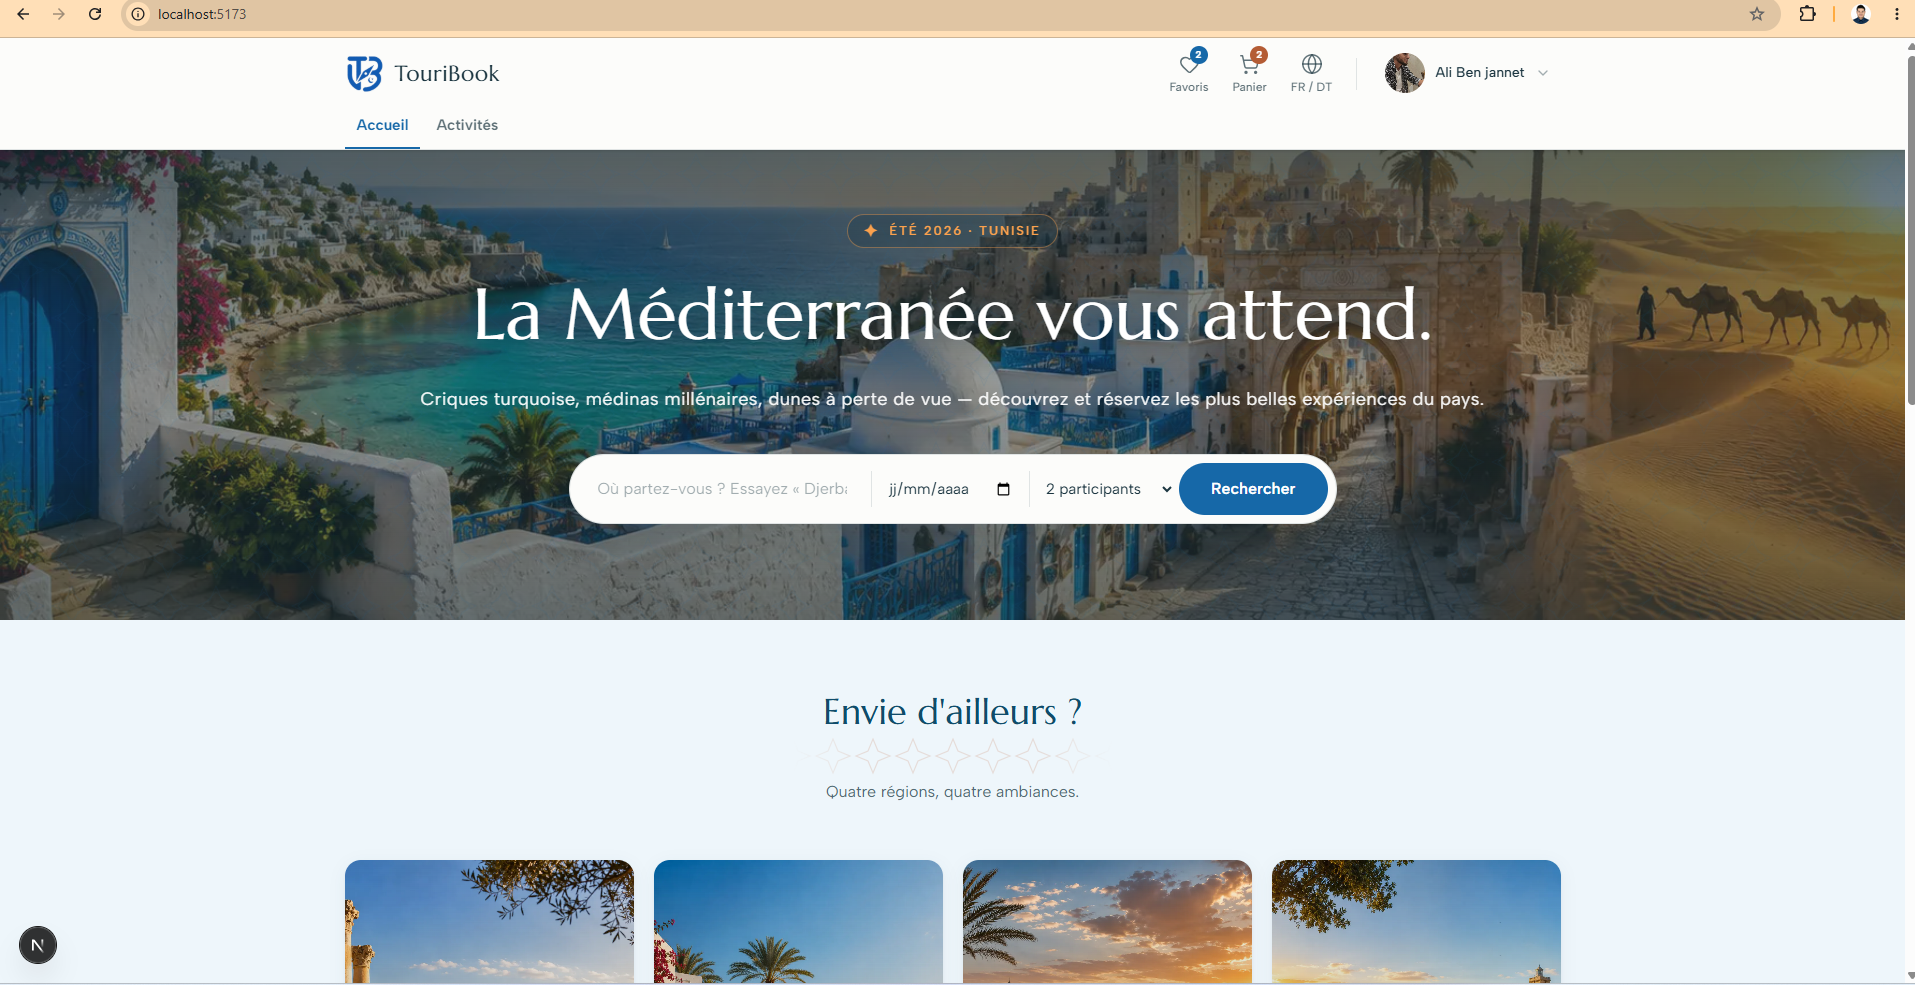
\includegraphics[width=0.92\textwidth]{screenshots/accueil.png}
\caption{Page d'accueil : bandeau de recherche, destinations mises en avant.}
\label{fig:accueil}
\end{figure}

\begin{figure}[htbp]
\centering
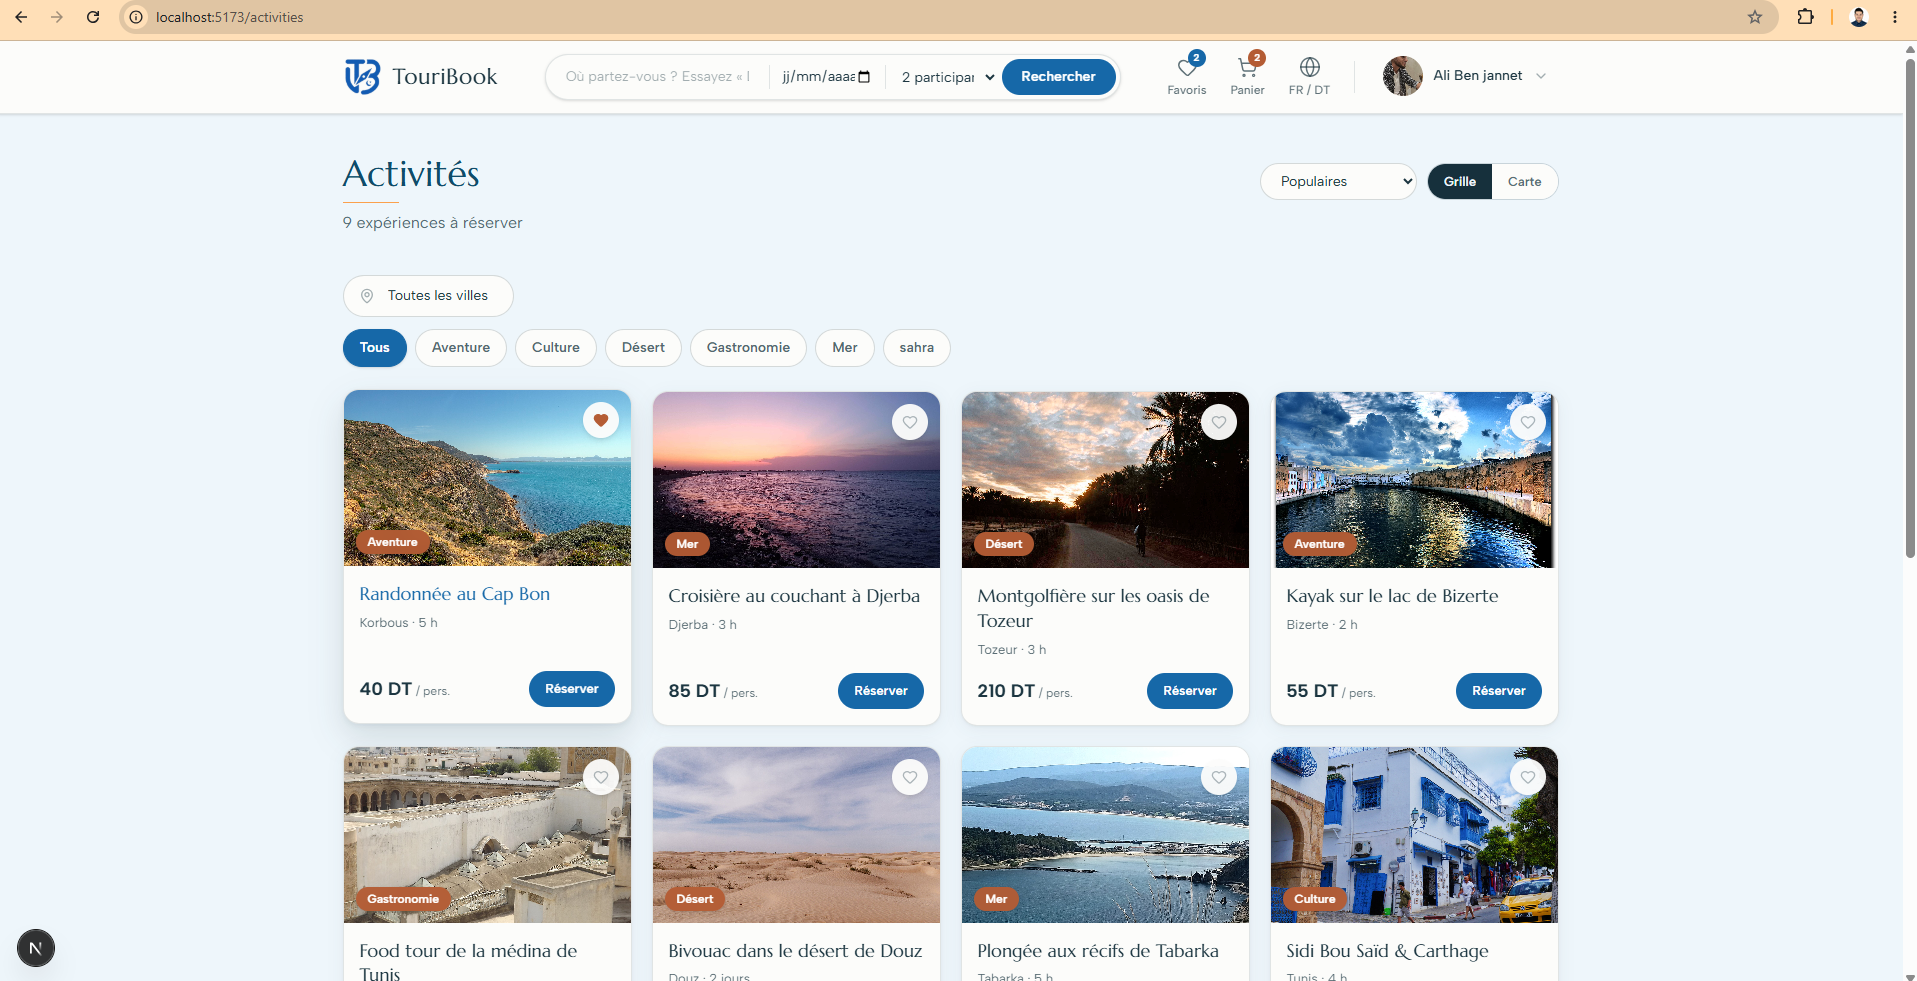
\includegraphics[width=0.92\textwidth]{screenshots/catalogue.png}
\caption{Catalogue : recherche instantanée, filtres par ville et catégorie.}
\label{fig:catalogue}
\end{figure}

\begin{figure}[htbp]
\centering
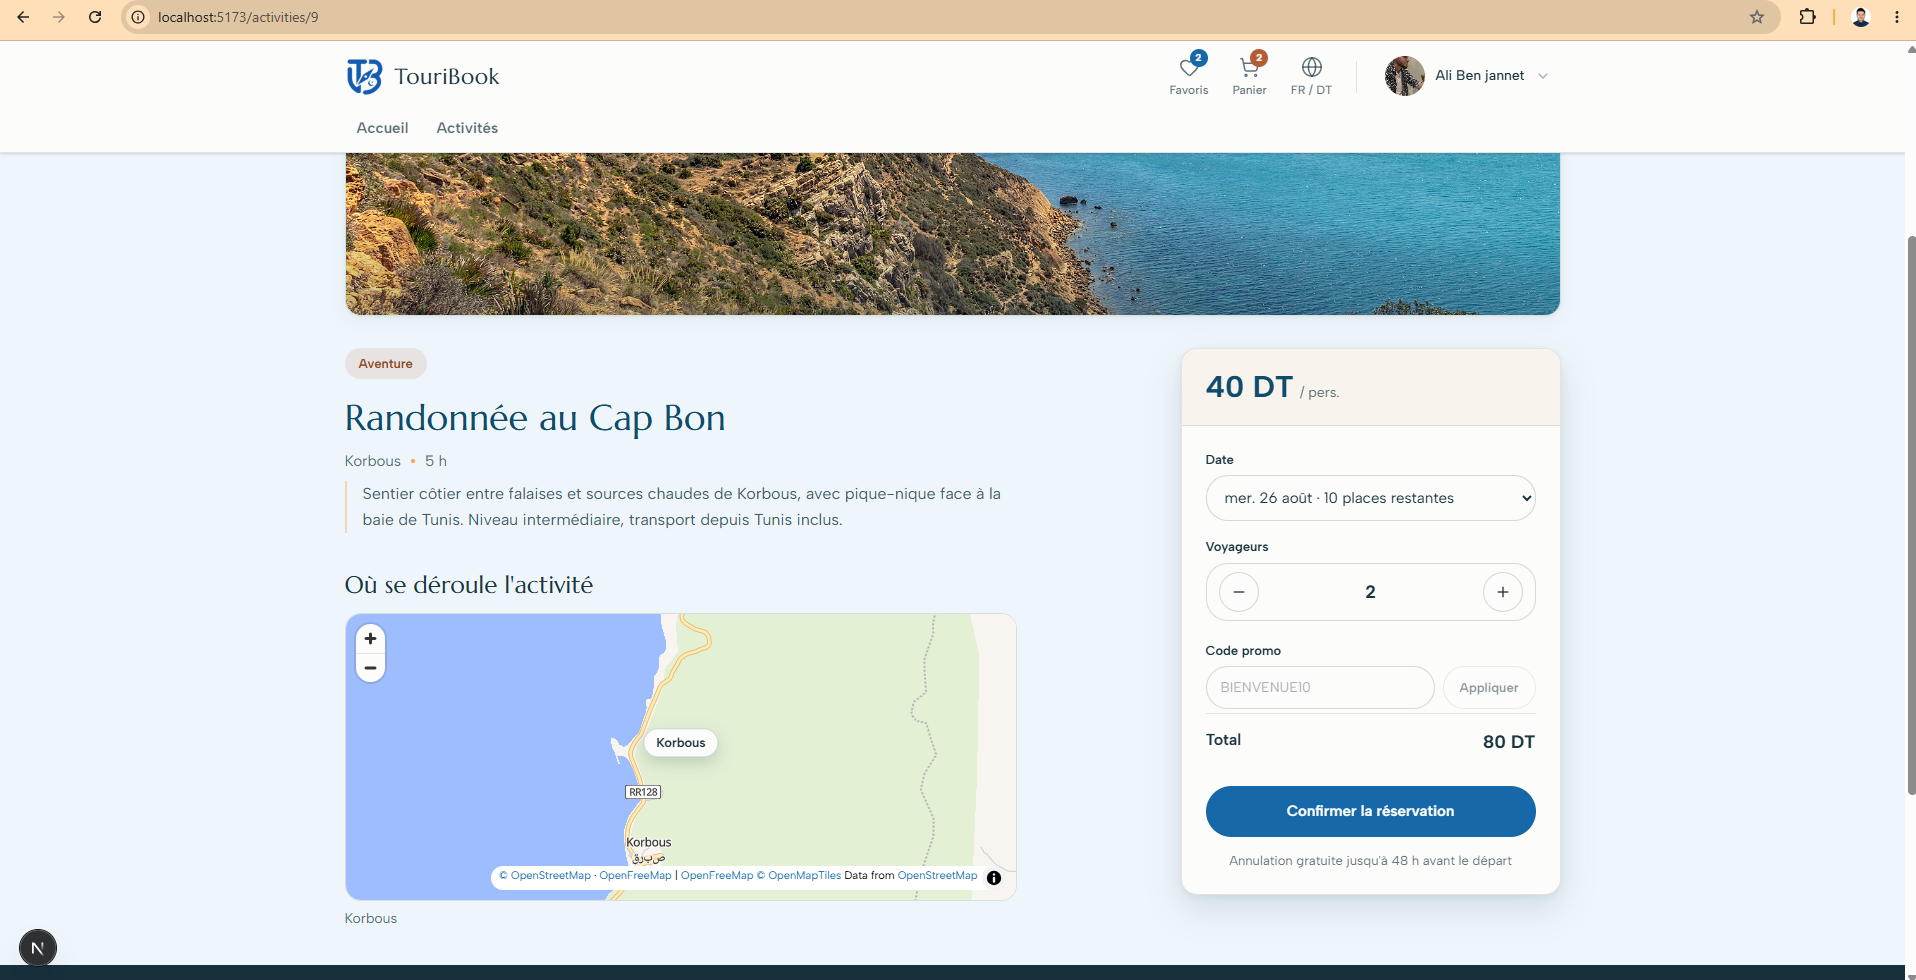
\includegraphics[width=0.92\textwidth]{screenshots/detail-activite.png}
\caption{Fiche d'activité : description, localisation et module de réservation.}
\label{fig:detail}
\end{figure}

\begin{figure}[htbp]
\centering
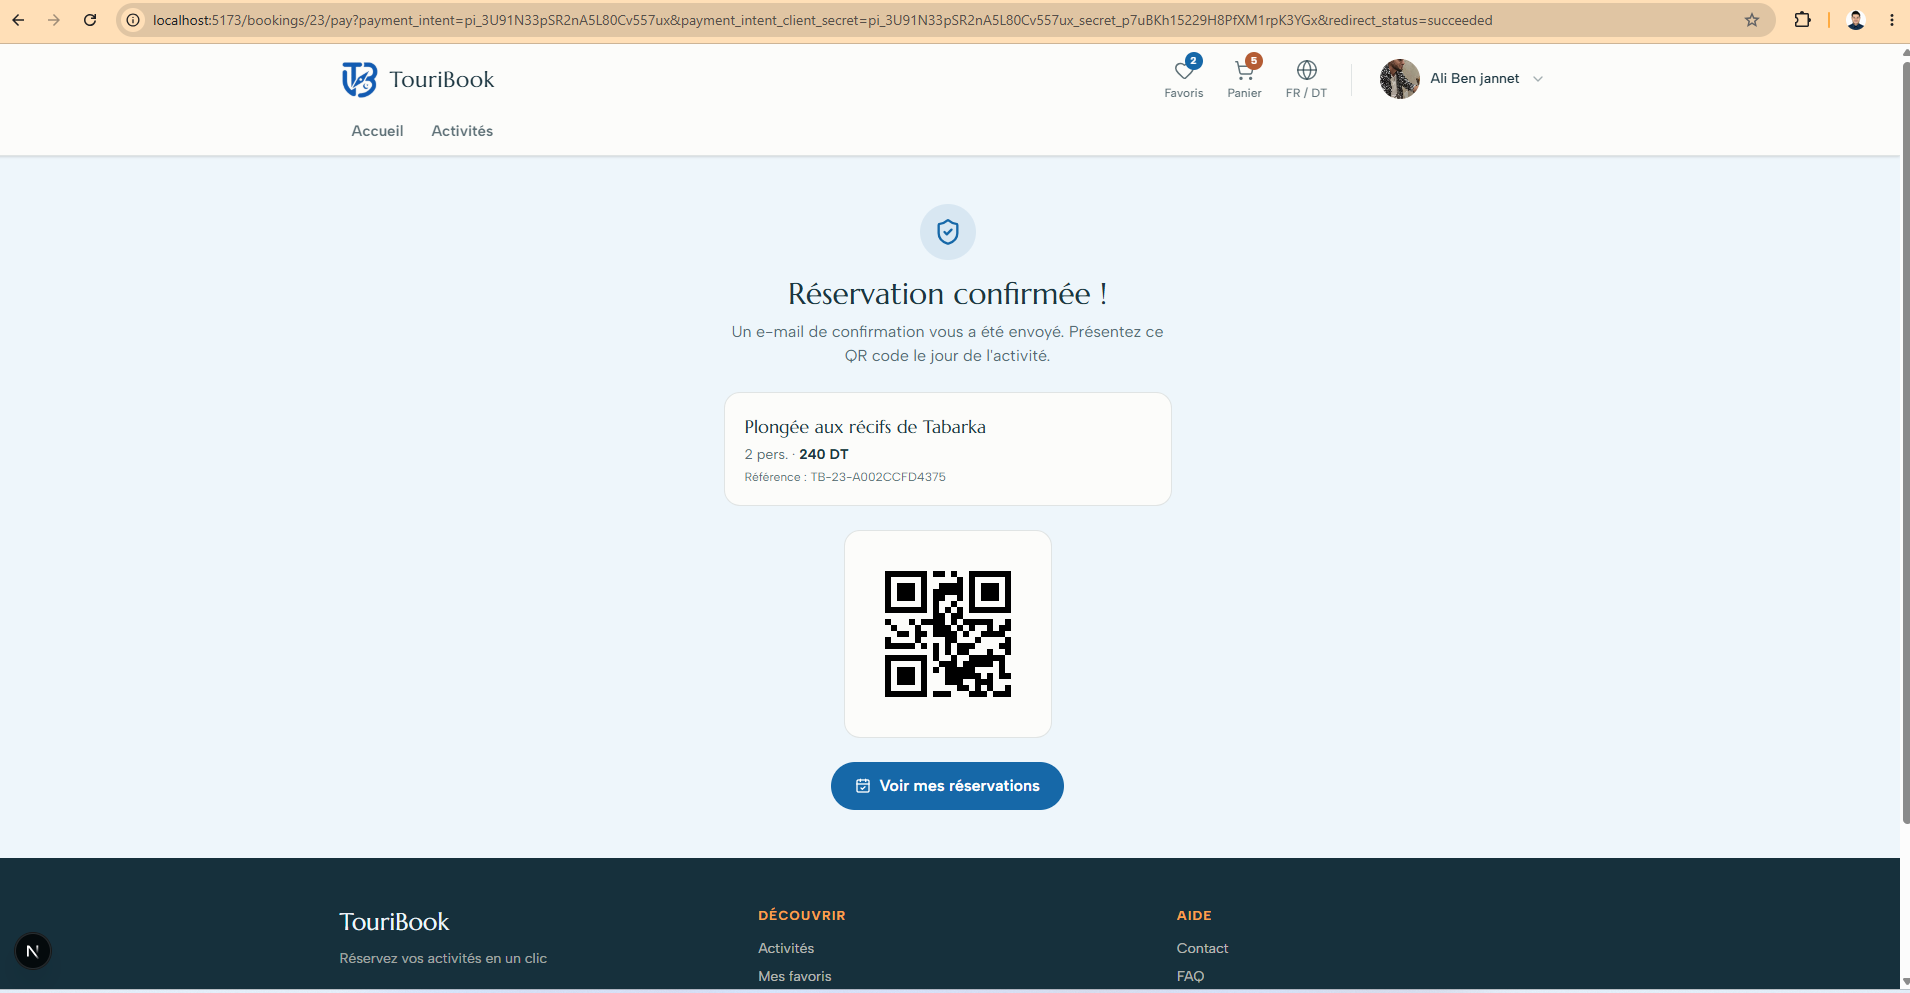
\includegraphics[width=0.92\textwidth]{screenshots/paiement-confirme.png}
\caption{Confirmation de réservation avec QR code de vérification.}
\label{fig:confirmation}
\end{figure}

\begin{figure}[htbp]
\centering
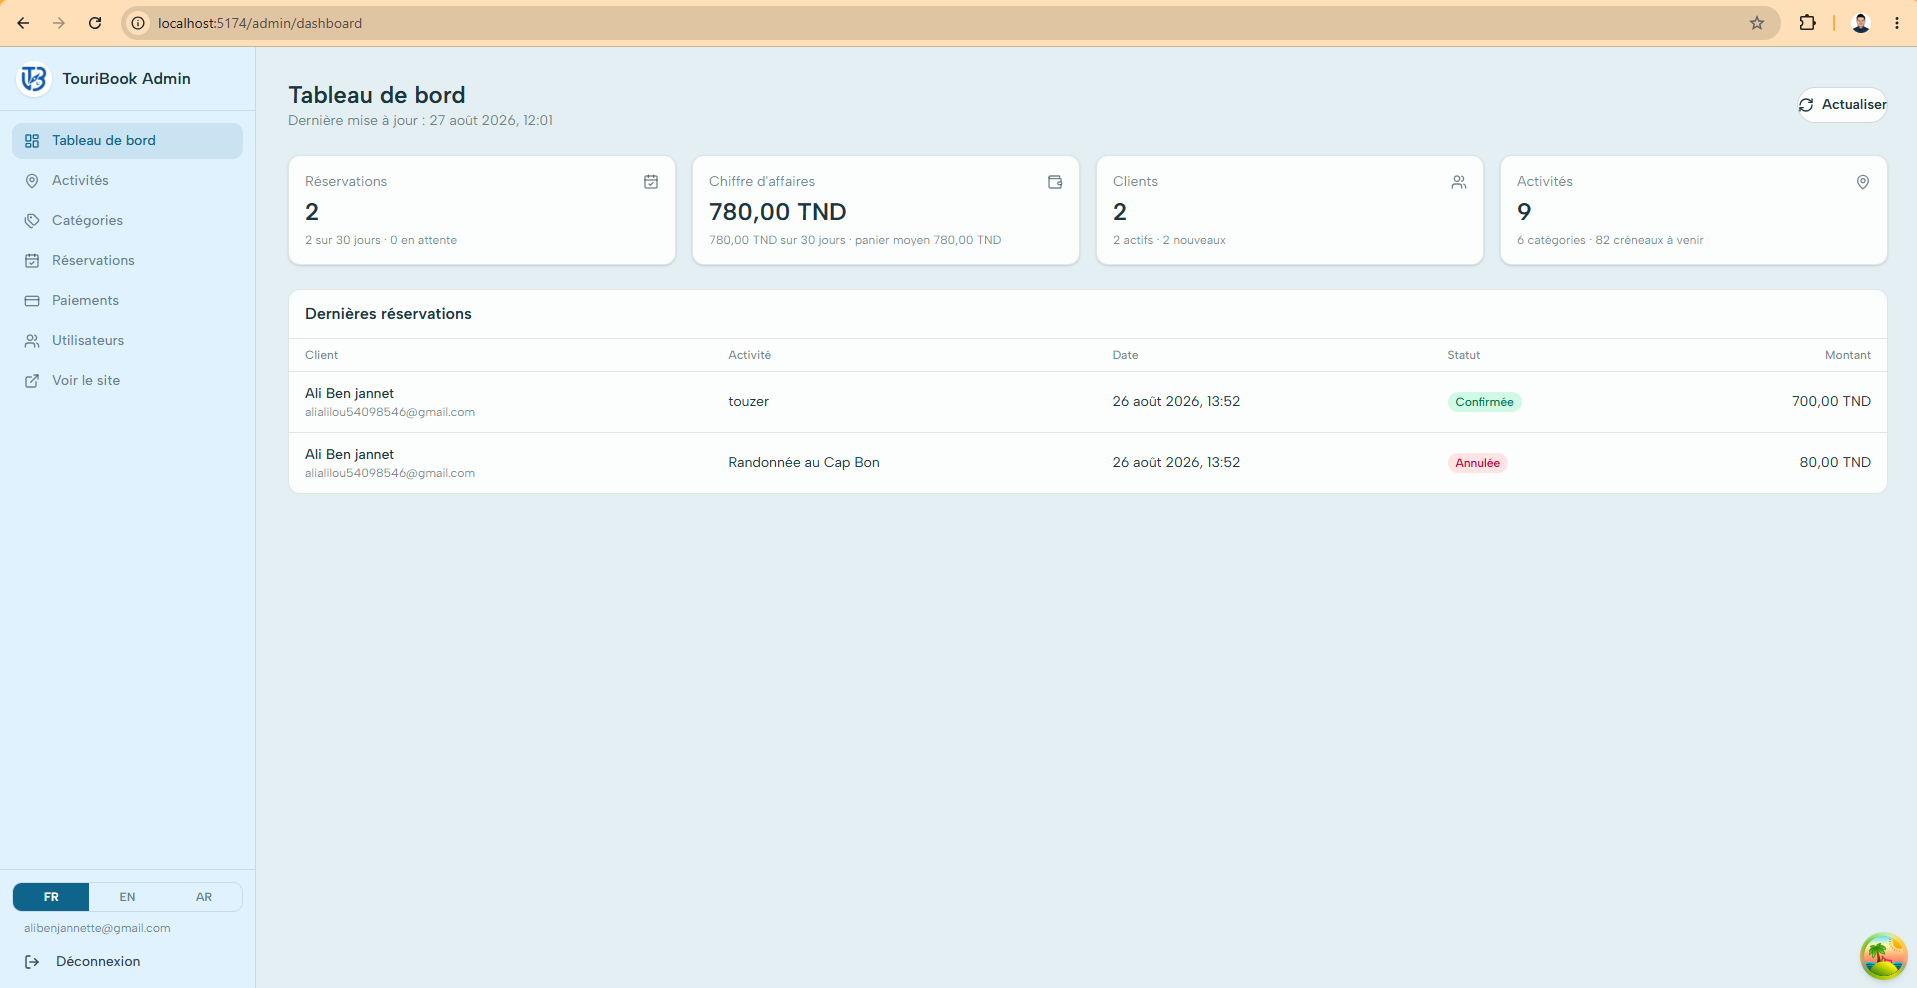
\includegraphics[width=0.92\textwidth]{screenshots/admin-dashboard.png}
\caption{Tableau de bord administrateur : indicateurs et dernières réservations.}
\label{fig:dashboard}
\end{figure}

% =====================================================================
\chapter{Sécurité}

\section{Authentification}

\begin{itemize}
  \item \textbf{Mots de passe} : hachés en \texttt{pbkdf2\_sha256}, jamais
    stockés en clair.
  \item \textbf{Jetons d'accès} : JWT de durée courte (30 minutes), validés
    localement par chaque service.
  \item \textbf{Jetons de rafraîchissement} : stockés hachés en SHA-256,
    révocables individuellement, ce qui permet de fermer une session à distance.
  \item \textbf{Vérification d'adresse} obligatoire avant toute connexion.
  \item \textbf{Limitation de débit} sur les routes sensibles (connexion,
    inscription, réinitialisation).
\end{itemize}

\section{Protection des routes internes}

Les routes \texttt{/internal/*}, utilisées pour la communication entre services,
sont protégées par une clé partagée et \textbf{ne sont jamais routées par la
passerelle}. Elles restent donc inaccessibles depuis l'extérieur.

\section{Anti-énumération}

Les réponses aux demandes de réinitialisation de mot de passe et de renvoi de
courriel sont identiques, que l'adresse existe ou non. Un attaquant ne peut pas
déduire quelles adresses sont enregistrées.

\section{Données personnelles}

La suppression de compte (\texttt{DELETE /auth/me}) anonymise les données
personnelles, révoque toutes les sessions et purge les jetons. Une page de
politique de confidentialité, accessible publiquement, détaille les données
collectées et les droits de l'utilisateur.

\section{Limites de sécurité assumées}

Deux points sont documentés comme des compromis conscients :

\begin{itemize}
  \item \textbf{Secret JWT partagé} : chaque service détient le secret de
    signature. Un service compromis pourrait forger un jeton administrateur. Ce
    risque est accepté dans le cadre d'un réseau interne de confiance ; une
    évolution vers RS256 avec clés asymétriques est documentée.
  \item \textbf{Clé interne unique} : tous les services partagent la même clé
    d'accès aux routes internes, ce qui empêche la traçabilité par appelant.
\end{itemize}

% =====================================================================
\chapter{Tests et qualité}

\section{État actuel}

\begin{longtable}{@{}p{6.4cm}p{8cm}@{}}
\toprule
\textbf{Élément} & \textbf{État} \\
\midrule
\endhead
Tests du parcours d'authentification & Implémentés (pytest, isolation par
transaction) \\
\addlinespace
Tests unitaires frontend & Implémentés (Vitest) \\
\addlinespace
Vérification de types TypeScript & Stricte, sans erreur sur les deux
applications et les paquets partagés \\
\addlinespace
Tests de concurrence & Validés par scripts dédiés (résultats au chapitre~5),
non encore formalisés en suite pytest \\
\addlinespace
Audit d'internationalisation & Automatisé — aucune clé manquante \\
\addlinespace
Vérification des contrastes & Automatisée — 12 combinaisons conformes WCAG AA \\
\addlinespace
Tests de bout en bout & Non implémentés \\
\addlinespace
Intégration continue & Non configurée \\
\bottomrule
\end{longtable}

\section{Analyse critique}

La couverture de tests constitue la principale faiblesse du projet. Les
mécanismes les plus délicats — concurrence, saga, expiration, réconciliation —
ont été validés expérimentalement, mais par des scripts de vérification plutôt
que par une suite de tests rejouable automatiquement.

Cette validation reste rigoureuse : chaque correctif de concurrence a été
précédé d'un test reproduisant le défaut, puis suivi d'un test confirmant sa
disparition. Le travail restant consiste à formaliser ces scripts en tests
pytest intégrés à une chaîne d'intégration continue.

% =====================================================================
\chapter{Difficultés rencontrées}

Ce chapitre présente les problèmes réellement rencontrés et la manière dont ils
ont été résolus.

\section{Cohérence entre deux bases sans transaction commune}

\textbf{Problème.} Décrémenter les places et créer la réservation concernent deux
bases distinctes ; une panne entre les deux opérations laisse le système
incohérent.

\textbf{Solution.} Saga orchestrée avec compensation, complétée par l'expiration
automatique et le script de réconciliation. Trois niveaux de protection qui se
complètent.

\section{Races conditions non détectées à l'usage}

\textbf{Problème.} Trois défauts de concurrence subsistaient dans le code après
la mise en place de la saga : l'annulation, la confirmation de paiement et la
création de réservation vérifiaient un état avant de l'écrire, sans atomicité.

Le cas de l'annulation était le plus grave : huit annulations simultanées de la
même réservation libéraient huit fois les places, créant sept places
inexistantes.

\textbf{Solution.} Toutes les transitions d'état passent désormais par un
\texttt{UPDATE} conditionnel, et l'unicité des réservations est garantie par un
index en base. Chaque correctif a été validé par un test reproduisant d'abord le
défaut.

\section{Rendu serveur et état côté client}

\textbf{Problème.} Le rendu côté serveur ignore le \texttt{localStorage} : le
serveur produisait une page en français et déconnectée, tandis que le premier
rendu du navigateur utilisait la langue mémorisée et la session restaurée. React
détectait la divergence et régénérait toute la page.

\textbf{Solution.} Un mécanisme différant l'application de l'état client jusqu'à
la fin de l'hydratation. Le traitement a été appliqué à la racine — dans le
fournisseur d'authentification et un hook de langue partagé — plutôt qu'au cas
par cas, ce qui couvre l'ensemble des composants concernés.

\section{Internationalisation du contenu métier}

\textbf{Problème.} Les fichiers de traduction ne peuvent pas traduire des
contenus saisis par l'administrateur. Titres et descriptions restaient en
français quelle que soit la langue choisie.

\textbf{Solution.} Colonnes de traduction en base, champs correspondants dans le
formulaire d'administration, et repli automatique sur le français. Un piège a dû
être traité : le formulaire ne rechargeait pas les traductions existantes en
mode édition, si bien qu'un simple enregistrement les aurait effacées.

\section{Langue des fonds cartographiques}

\textbf{Problème.} Les tuiles cartographiques images affichent les noms de lieux
dans la langue locale — en arabe pour la Tunisie — sans possibilité de
changement.

\textbf{Solution.} Après vérification de plusieurs fournisseurs, aucun service de
tuiles images ne permet de choisir la langue : le texte est gravé dans l'image.
Le passage aux tuiles vectorielles, où les libellés sont des données stylées à
l'affichage, était la seule solution.

\section{Décalage de fuseau horaire}

\textbf{Problème.} La colonne d'horodatage des réservations est de type
\emph{timestamp sans fuseau} et contient de l'UTC, alors que le serveur de
développement est en UTC+1.

\textbf{Solution.} Vérification empirique du contenu réel de la base avant
d'écrire la comparaison. Utiliser l'heure locale aurait déclenché les
expirations une heure trop tôt — un défaut invisible en test et difficile à
diagnostiquer en production.

% =====================================================================
\chapter{Perspectives}

\section{Court terme}

\begin{itemize}
  \item \textbf{Suite de tests automatisée} : formaliser les scripts de
    validation en tests pytest, et mettre en place une chaîne d'intégration
    continue.
  \item \textbf{Test de bout en bout} : automatiser le parcours nominal complet,
    de l'inscription au QR code.
  \item \textbf{Délais et reprises} sur les appels inter-services, aujourd'hui
    sans temporisation ni nouvelle tentative.
  \item \textbf{Corrélation des journaux} : propager un identifiant de requête à
    travers les services pour faciliter le diagnostic.
\end{itemize}

\section{Moyen terme}

\begin{itemize}
  \item \textbf{Recommandations} : suggestions d'activités similaires par règles
    métier (même catégorie, prix proche), puis recommandations selon
    l'historique. Une approche par apprentissage automatique n'est pas
    justifiée tant que le volume de données reste faible.
  \item \textbf{Panier multi-activités} et paiement groupé.
  \item \textbf{Remboursement} via l'API Stripe lors de l'annulation d'une
    réservation payée.
  \item \textbf{Référencement multilingue} : routes par langue et balises
    \texttt{hreflang}.
\end{itemize}

\section{Long terme}

\begin{itemize}
  \item Signature asymétrique des jetons (RS256), supprimant le secret partagé.
  \item Migrations versionnées généralisées à tous les services.
  \item File de messages pour les notifications, aujourd'hui au mieux
    « meilleur effort ».
  \item Observabilité complète : traces distribuées et journalisation
    centralisée.
\end{itemize}

% =====================================================================
\chapter{Conclusion}

TouriBook livre une plateforme de réservation fonctionnelle de bout en bout,
depuis la découverte d'une activité jusqu'au justificatif de réservation, avec
un espace d'administration complet et une interface disponible en trois langues.

Sur le plan technique, l'intérêt du projet réside moins dans les fonctionnalités
que dans les problèmes que l'architecture distribuée a imposé de résoudre.
Garantir qu'aucune place ne soit vendue deux fois, alors que la vérification et
l'écriture concernent deux bases sans transaction commune, a exigé une démarche
rigoureuse : reproduire d'abord le défaut par un test, puis corriger, puis
vérifier la correction. Trois défauts de concurrence réels ont ainsi été
identifiés et éliminés — dont un qui créait des places à partir de rien.

Le projet assume ses limites. La couverture de tests reste insuffisante et
l'intégration continue n'est pas en place ; ces manques sont identifiés et
documentés plutôt que dissimulés. De même, les fonctionnalités non implémentées
— recommandations, panier, remboursement — sont présentées comme des
perspectives et non comme des acquis.

Cette démarche — mesurer avant d'affirmer, documenter les compromis, distinguer
ce qui est fait de ce qui reste à faire — constitue sans doute l'apport le plus
durable de ce travail.

\end{document}
